\documentclass{article}

\usepackage{enumitem}
\usepackage{amsmath}
\usepackage{tikz}

\begin{document}
% Exercice 18 Cycle 4 Myriade
Trois chats se précipitent sur une assiette de nourriture. Le premier dévore
le quart de l'assiette, le deuxième en dévore les trois huitièmes.
\begin{enumerate}
    \item Calculer la fraction de l'assiette dévorée par les deux premiers
    chats.
    \item Quelle est la part du troisième chat~?
\end{enumerate}
% Exercice 19 Cycle 4 Myriade
Dans la classe de 4$^{\text{e}}$ B, la moitié des élèves vient en bus, un
dixième des élèves arrive en voiture et un cinquième des élèves vient à pied.
Les autres élèves viennent à vélo.
\begin{enumerate}
    \item Quelle fraction d'élèves de cette classe vient au collège en
    utilisant un véhicule à moteur~?
    \item Quelle fraction d'élèves de cette classe vient au collège à pied
    ou à vélo~?
    \item Quelle fraction d'élèves de cette classe vient au collège à vélo~?
\end{enumerate}
% Exercice 21 Cycle 4 Myriade
{\centering Cycle4Myriade83-21pic\par}
Le tour de France 2015 comportait 21 étapes~:
\begin{itemize}[label=$-$]
    \item neuf étapes de plaines~;
    \item des étapes accidentées~;
    \item des étapes de montagne~;
    \item une étape en contre-la-montre en individuel~;
    \item une étape en contre-la-montre par équipe.
\end{itemize}
\begin{enumerate}
    \item Un septième des étapes était sur le parcours accidenté contre trois
    septièmes en plaines.\par Combien y a-t-il eu d'étapes accidentées~?
    \item Quelle fraction du nombre total d'étapes correspond aux étapes de
    montagne~?
\end{enumerate}
% Exercice 8 p. 85 Cycle 4 Myriade
Le rectangle ABCD est tel que $\text{AB}=\dfrac{17}3$ cm et
$\text{BC}=\dfrac45$ cm.\par\medskip\noindent
Calculer le périmètre de ce rectangle.
% Exercice 13 Cycle 4 Myriade p. 85
Compléter cette pyramide de façon à ce que le nombre figurant dans chaque case
soit égal à la somme des nombres figurant dans les deux cases sur lesquelles
elle repose.\par\smallskip\noindent
{\centering
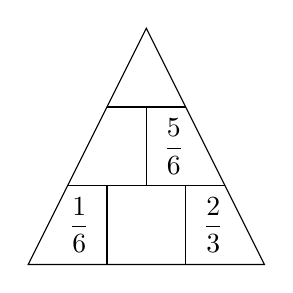
\begin{tikzpicture}
    \coordinate(A0)at(0,0);
    \coordinate(A1)at(1,0);
    \coordinate(A2)at(2,0);
    \coordinate(A3)at(3,0);
    \coordinate(B0)at(1/2,1);
    \coordinate(B1)at(1,1);
    \coordinate(B2)at(1.5,1);
    \coordinate(B3)at(2,1);
    \coordinate(B4)at(2.5,1);
    \coordinate(C0)at(1,2);
    \coordinate(C1)at(1.5,2);
    \coordinate(C2)at(2,2);
    \coordinate(D0)at(1.5,3);
    \draw(A0)--(A3)--(D0)--cycle;
    \draw(B0)--(B4);
    \draw(C0)--(C2);
    \draw(C1)--(B2);
    \draw(B1)--(A1);
    \draw(B3)--(A2);
    \draw node at(0.65,0.5){$\dfrac16$};
    \draw node at(2.35,0.5){$\dfrac23$};
    \draw node at(1.85,1.5){$\dfrac56$};
\end{tikzpicture}
\par}
\end{document}